\documentclass[twoside]{book}

% Packages required by doxygen
\usepackage{calc}
\usepackage{doxygen}
\usepackage{graphicx}
\usepackage[utf8]{inputenc}
\usepackage{makeidx}
\usepackage{multicol}
\usepackage{multirow}
\usepackage{textcomp}
\usepackage[table]{xcolor}

% Font selection
\usepackage[T1]{fontenc}
\usepackage{mathptmx}
\usepackage[scaled=.90]{helvet}
\usepackage{courier}
\usepackage{amssymb}
\usepackage{sectsty}
\renewcommand{\familydefault}{\sfdefault}
\allsectionsfont{%
  \fontseries{bc}\selectfont%
  \color{darkgray}%
}
\renewcommand{\DoxyLabelFont}{%
  \fontseries{bc}\selectfont%
  \color{darkgray}%
}

% Page & text layout
\usepackage{geometry}
\geometry{%
  a4paper,%
  top=2.5cm,%
  bottom=2.5cm,%
  left=2.5cm,%
  right=2.5cm%
}
\tolerance=750
\hfuzz=15pt
\hbadness=750
\setlength{\emergencystretch}{15pt}
\setlength{\parindent}{0cm}
\setlength{\parskip}{0.2cm}
\makeatletter
\renewcommand{\paragraph}{%
  \@startsection{paragraph}{4}{0ex}{-1.0ex}{1.0ex}{%
    \normalfont\normalsize\bfseries\SS@parafont%
  }%
}
\renewcommand{\subparagraph}{%
  \@startsection{subparagraph}{5}{0ex}{-1.0ex}{1.0ex}{%
    \normalfont\normalsize\bfseries\SS@subparafont%
  }%
}
\makeatother

% Headers & footers
\usepackage{fancyhdr}
\pagestyle{fancyplain}
\fancyhead[LE]{\fancyplain{}{\bfseries\thepage}}
\fancyhead[CE]{\fancyplain{}{}}
\fancyhead[RE]{\fancyplain{}{\bfseries\leftmark}}
\fancyhead[LO]{\fancyplain{}{\bfseries\rightmark}}
\fancyhead[CO]{\fancyplain{}{}}
\fancyhead[RO]{\fancyplain{}{\bfseries\thepage}}
\fancyfoot[LE]{\fancyplain{}{}}
\fancyfoot[CE]{\fancyplain{}{}}
\fancyfoot[RE]{\fancyplain{}{\bfseries\scriptsize Generated on Wed May 6 2015 13\-:00\-:56 for My Project by Doxygen }}
\fancyfoot[LO]{\fancyplain{}{\bfseries\scriptsize Generated on Wed May 6 2015 13\-:00\-:56 for My Project by Doxygen }}
\fancyfoot[CO]{\fancyplain{}{}}
\fancyfoot[RO]{\fancyplain{}{}}
\renewcommand{\footrulewidth}{0.4pt}
\renewcommand{\chaptermark}[1]{%
  \markboth{#1}{}%
}
\renewcommand{\sectionmark}[1]{%
  \markright{\thesection\ #1}%
}

% Indices & bibliography
\usepackage{natbib}
\usepackage[titles]{tocloft}
\setcounter{tocdepth}{3}
\setcounter{secnumdepth}{5}
\makeindex

% Hyperlinks (required, but should be loaded last)
\usepackage{ifpdf}
\ifpdf
  \usepackage[pdftex,pagebackref=true]{hyperref}
\else
  \usepackage[ps2pdf,pagebackref=true]{hyperref}
\fi
\hypersetup{%
  colorlinks=true,%
  linkcolor=blue,%
  citecolor=blue,%
  unicode%
}

% Custom commands
\newcommand{\clearemptydoublepage}{%
  \newpage{\pagestyle{empty}\cleardoublepage}%
}


%===== C O N T E N T S =====

\begin{document}

% Titlepage & ToC
\hypersetup{pageanchor=false}
\pagenumbering{roman}
\begin{titlepage}
\vspace*{7cm}
\begin{center}%
{\Large My Project }\\
\vspace*{1cm}
{\large Generated by Doxygen 1.8.6}\\
\vspace*{0.5cm}
{\small Wed May 6 2015 13:00:56}\\
\end{center}
\end{titlepage}
\clearemptydoublepage
\tableofcontents
\clearemptydoublepage
\pagenumbering{arabic}
\hypersetup{pageanchor=true}

%--- Begin generated contents ---
\chapter{Optimization Schemes}
\label{optschemes}
\hypertarget{optschemes}{}
\hypertarget{tut-xo_Contents}{}\section{Contents}\label{tut-xo_Contents}

\begin{DoxyItemize}
\item \hyperlink{optschemes_overview}{Overview\-: What are optimimization schemes, and why use them?}
\begin{DoxyItemize}
\item \hyperlink{optschemes_quick-over}{In a nutshell..}
\item \hyperlink{optschemes_detailed-over}{More details}
\end{DoxyItemize}
\item \hyperlink{optschemes_gui}{Optimization scheme user interface}
\begin{DoxyItemize}
\item \hyperlink{optschemes_gui-list}{Optimization step list}
\item \hyperlink{optschemes_gui-add}{Add new optimization step}
\item \hyperlink{optschemes_gui-rem}{Remove current optimization step}
\item \hyperlink{optschemes_gui-tselect}{Select template}
\item \hyperlink{optschemes_gui-editor}{Template editor}
\item \hyperlink{optschemes_gui-save}{Save scheme}
\item \hyperlink{optschemes_gui-load}{Resume scheme}
\end{DoxyItemize}
\item \hyperlink{optschemes_creating}{How to build an optimization scheme?}
\item \hyperlink{optschemes_saving}{How to save an optimization scheme for later?}
\item \hyperlink{optschemes_loading}{How to load an optimization scheme?}
\item \hyperlink{optschemes_format}{What is saved?}
\item \hyperlink{optschemes_suggest}{Suggestions for optimization schemes}
\begin{DoxyItemize}
\item \hyperlink{optschemes_sug-xtal}{Crystals (Xtal\-Opt)}
\end{DoxyItemize}
\end{DoxyItemize}\hypertarget{optschemes_overview}{}\section{Overview\-: What are optimimization schemes, and why use them?}\label{optschemes_overview}
\hypertarget{optschemes_quick-over}{}\subsection{In a nutshell..}\label{optschemes_quick-over}
An optimization scheme is a series of optimization steps (\char`\"{}optsteps\char`\"{}) that are to be performed in sequence on a structure. Each optimization step consists of a set of input file templates for the queuing system and optimizer to be used, and the structure is updated after each completes. So if an optimization scheme contains three optimization steps, a stucture's lifecycle is\-:


\begin{DoxyEnumerate}
\item Generation of initial structure
\item Perform optstep 1 on initial structure
\item Update structure from the results of optstep 1
\item Perform optstep 2 on current structure (result of optstep 1)
\item Update structure from the results of optstep 2
\item Perform optstep 3 on current structure (result of optstep 2)
\item Update structure from the results of optstep 3
\item Current structure (result of optstep 3) is either accepted into the breeding pool or discarded, depending on its enthalpy relative to the other optimized structures.
\end{DoxyEnumerate}\hypertarget{optschemes_detailed-over}{}\subsection{More details}\label{optschemes_detailed-over}
The efficiency of searching a potential energy surface for a global minimum can be significantly improved by moving each candidate structure to the nearest local minimum, i.\-e. performing a geometry optimization. The differences between searching with and without carrying out these local optimizations are explored in detail in Woodley S\-M, Catlow C\-R\-A. Comp. Mat. Sci. 2009;45(1)\-:84-\/95 (Available at\-: \href{http://linkinghub.elsevier.com/retrieve/pii/S0927025608003030}{\tt http\-://linkinghub.\-elsevier.\-com/retrieve/pii/\-S0927025608003030} ).

Why not just perform a single geometry optimization on each structure? Stochastic search techniques, such as Xtal\-Opt, will often need to perform geometry optimizations on structures that are far from a stationary point on the potential energy surface. For example, the randomly generated structures in the first generation of an evolutionary search are often highly disordered with unrealistic atomic separations. If these structures were to be optimized in a single step with accurately small convergence criteria, it would be quite expensive. Also, it is more than likely that most of the optimizations would not finish successfully before reaching the maximum number of geometry steps allowed by the optimizer or specified in the input. A second issue is that complex structures (periodic crystals, for example) often have so many degrees of freedom that convergence in a single step is difficult from a poor starting point (consider the effect on atomic coordinates when a unit cell's translation vector is modified).

The first problem (effectively optimizing to small convergence) can be solved by implementing an optimization scheme that optimizes to successively smaller convergence cutoffs.

The second problem can be addressed by reducing the degrees of freedom in the early optsteps and only optimizing everything once each component has individually converged to a reasonable parameterization. See \hyperlink{optschemes_suggest}{Suggestions for optimization schemes} for examples.\hypertarget{optschemes_gui}{}\section{Optimization scheme user interface}\label{optschemes_gui}
 
\begin{DoxyImage}
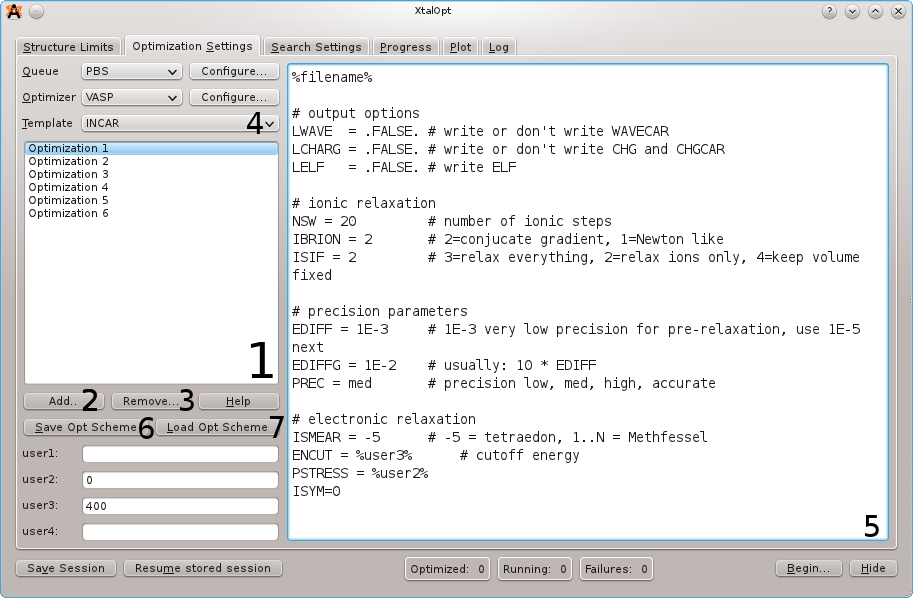
\includegraphics{optschemes-numberededitor.png}
\caption{width=}
\end{DoxyImage}


We will use the above screenshot as we describe the process of creating, saving, and loading optimization schemes. The numbers indicate\-:


\begin{DoxyEnumerate}
\item List of optimization steps
\item Button to add new optimization step
\item Button to remove current optimization step
\item Template selection menu
\item Template editor
\item Button to save current optimization scheme to file
\item Button to load optimization scheme from file
\end{DoxyEnumerate}\hypertarget{optschemes_gui-list}{}\subsection{Optimization step list}\label{optschemes_gui-list}
This list shows the currently available optimization steps in the order that they will be performed. The optstep that is currently selected for editing is highlighted, and the editable optstep can be selected by clicking the appropriate entry.\hypertarget{optschemes_gui-add}{}\subsection{Add new optimization step}\label{optschemes_gui-add}
Clicking this button will append a new optimization step to the optstep list. The new optstep's templates will be copies of the currently selected optstep's templates.\hypertarget{optschemes_gui-rem}{}\subsection{Remove current optimization step}\label{optschemes_gui-rem}
Click this button to delete the currently selected optimization step.\hypertarget{optschemes_gui-tselect}{}\subsection{Select template}\label{optschemes_gui-tselect}
This menu contains the filenames of the templates that are required by the currently selected queuing system (e.\-g. P\-B\-S, S\-G\-E, local...) and optimizer. The currently selected template is displayed in the template editor, and selecting a different template will update the editor.\hypertarget{optschemes_gui-editor}{}\subsection{Template editor}\label{optschemes_gui-editor}
This text editor is used to view and edit the currently selected template for the current optstep.\hypertarget{optschemes_gui-save}{}\subsection{Save scheme}\label{optschemes_gui-save}
This button will prompt for a location to save a .scheme file containing the current optimization step.\hypertarget{optschemes_gui-load}{}\subsection{Resume scheme}\label{optschemes_gui-load}
This button will prompt for an existing .scheme file to load.\hypertarget{optschemes_creating}{}\section{How to build an optimization scheme?}\label{optschemes_creating}
Creating a working scheme from scratch may take some time. We recommend checking the samples/ directory of the source code to obtain sample scheme for each optimizer (see \hyperlink{optschemes_loading}{How to load an optimization scheme?}) and verifying that they are appropriate for the system under consideration before starting a search.

If there is not an appropriate sample, the following prescription may be used to generate your own\-:


\begin{DoxyEnumerate}
\item Generate a random structure of the system under consideration. This may be done by hand, or by running a search just long enough to create the first random generation and saving one of the structures.
\item Create a starting optstep with the desired convergence criteria
\item Manually submit the optimization
\item If the optimization fails\-:
\begin{DoxyEnumerate}
\item First determine why -- if the maximum iterations were exceeded or the optimization was aborted due to a badly performing minimizer, try one of the ideas below. Other optimization problems are beyond the scope of this document.
\item Reduce the convergence criteria of the current trial optstep
\item Remove degrees of freedom, e.\-g. by fixing cell parameters, atomic positions, etc
\item Reduce the accuracy of the calculation in other ways (use a courser integration grid, etc).
\item Change the minimizer (e.\-g. tell the optimizer to use conjugate gradients rather than B\-F\-G\-S, etc)
\end{DoxyEnumerate}
\item Once the optimization succeeds, create another set of input files with the desired convergence criteria for all degrees of freedom.
\item Manually submit the new optimization step. If it fails, try the ideas above until it converges.
\item Once the structure has converged to the desired level of accuracy, try to optimize another randomly generated structure using the optsteps that succeeded previously. Refine them if needed.
\item Once you have successfully optimized enough random structures that you are confident in your method, gather all of the inputs used and write your scheme from them.
\end{DoxyEnumerate}

The scheme may be written by copying each input file into the template editor (with the appropriate optstep and template selected, of course) and replacing the structure-\/specific information with the appropriate keywords. Click the \char`\"{}\-Help\char`\"{} button for the complete list of keywords.

We have found that the optimization schemes are surprisingly transferable within an optimizer, so once you have a working optimization scheme for a given optimization code only minor tweaks (usually to the energy cutoffs, etc ) are necessary to use it on a different chemical system.\hypertarget{optschemes_saving}{}\section{How to save an optimization scheme for later?}\label{optschemes_saving}
Once you have written your optimization scheme, you will want to save it for fast retrieval later (otherwise you will need to copy/paste and edit all of the templates again!). To save, simply click the \char`\"{}\-Save Opt
\-Scheme\char`\"{} button and enter an appropriate filename with an extension of .scheme.\hypertarget{optschemes_loading}{}\section{How to load an optimization scheme?}\label{optschemes_loading}
Loading an optimization is quite simple -- just click the \char`\"{}\-Load Opt
\-Scheme\char`\"{} button and select the .scheme file you wish to load. This will also update the current queuing system and optimizer to those specified by the scheme.\hypertarget{optschemes_format}{}\section{What is saved?}\label{optschemes_format}
The optimization scheme files contain more than just the templates for each optstep. They also store queue and optimizer specific settings. This is useful for storing configuration options for different clusters along with the scheme. Note that although Xtal\-Opt will prompt for an S\-S\-H password if needed, it is {\bfseries N\-O\-T} stored in the scheme file.\hypertarget{optschemes_suggest}{}\section{Suggestions for optimization schemes}\label{optschemes_suggest}
\hypertarget{optschemes_sug-xtal}{}\subsection{Crystals (\-Xtal\-Opt)}\label{optschemes_sug-xtal}
The following list describes the optimization steps used in the samples/vasp-\/xtalopt.\-scheme file distributed with the Xtal\-Opt source code\-:
\begin{DoxyEnumerate}
\item Fix unit cell, only optimize atomic coordinates. A very loose convergence criterion is used, and the number of K\-P\-O\-I\-N\-Ts is kept small.
\item The cell volume is fixed, but atomic positions and cell parameters are allowed to vary. The convergence criteria is the same as before, as is the K\-P\-O\-I\-N\-T grid.
\item All degrees of freedom are considered using the same convergence criteria as before, but with a finer K\-P\-O\-I\-N\-T grid.
\item Same as before, but with a stricter convergence criteria.
\item Same as before, but with a stricter convergence criteria and more K\-P\-O\-I\-N\-Ts.
\item Same as before, but with more K\-P\-O\-I\-N\-Ts.
\end{DoxyEnumerate}

This is only one of many possible optimization schemes that may work for crystals. It may need to be modified to work for your particular system. 
%--- End generated contents ---

% Index
\newpage
\phantomsection
\addcontentsline{toc}{chapter}{Index}
\printindex

\end{document}
